\chapter{TESTING AND EVALUATION}\label{chap:TESTING AND EVALUATION}
\hspace{0.5in}This chapter describes how we perform the usability testing to compare the time requirements between using an image retouching tool and the Face Replacement System, score the user satisfaction, and evaluate user interface. We also conducted an output evaluation to score the output satisfaction.

\section{Usability Testing}
\hspace{0.5in}We performed this testing by comparing the time to do face replacement between retouches by using the image retouching tool and the Face Replacement System. We selected the popular image retouching tool, Adobe Photoshop. We invited 7 volunteers who are our ICT friends and have experience, but not expertise, in Adobe Photoshop to perform this testing. The machine we used for this testing was a Dell Optiplex 330, using Intel Core2Duo E8400 3.0 GHz with 2 GB of RAM. The test volunteers had to replace faces from the images they had selected on their own by firstly using Adobe Photoshop, then using the Face Replacement System. Then, we recorded the time the volunteers spent for replacing faces using Adobe Photoshop and the time spent using the Face Replacement System.

After finishing this testing, the volunteers had to score their user satisfaction, which depended on the time requirements and the output images they created from using both Adobe Photoshop and the Face Replacement System. A percentage score was based on our four scales of measurement; Unacceptable (0\%), Acceptable (33.33\%), Good (66.67\%), and Perfect (100\%).

From this testing, the mean average required time for using Adobe Photoshop was 623.29 seconds, whereas the mean average required time for using the Face Replacement System was 245.43 seconds.

\begin{figure}[htb]
   \centering
   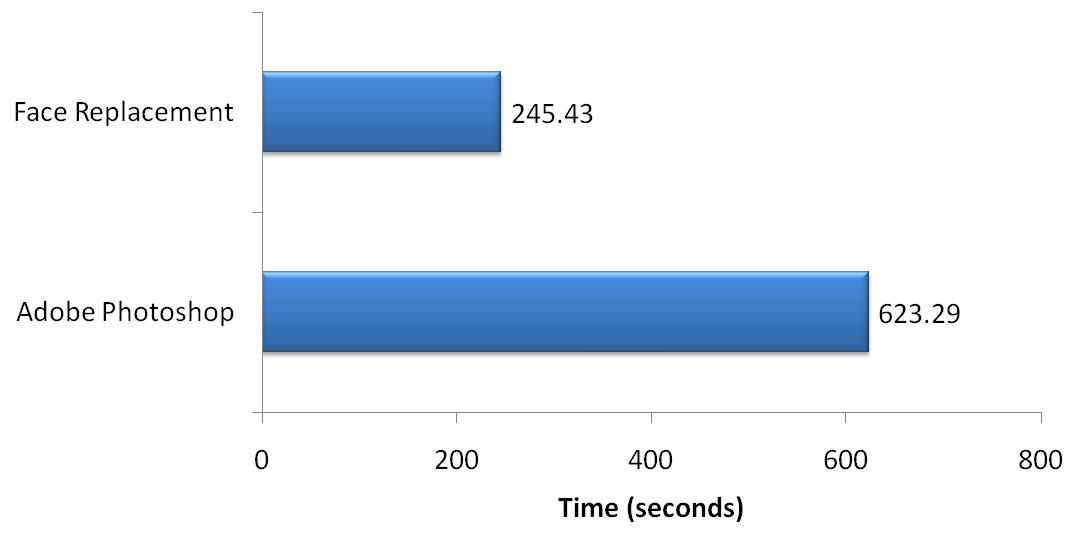
\includegraphics[width=12cm]{spendingtime.png}
   \caption{The Graph Shows the Mean Average Required Time for both Adobe Photoshop and the Face Replacement System}
   \label{fig:SpendingTime}
\end{figure}

For the user satisfaction, the mean average satisfaction score for Adobe Photoshop was 47\% (in Acceptable level), whereas the mean average satisfaction score for the Face Replacement System was 70 \% (in Good level).

\begin{figure}[htb]
   \centering
   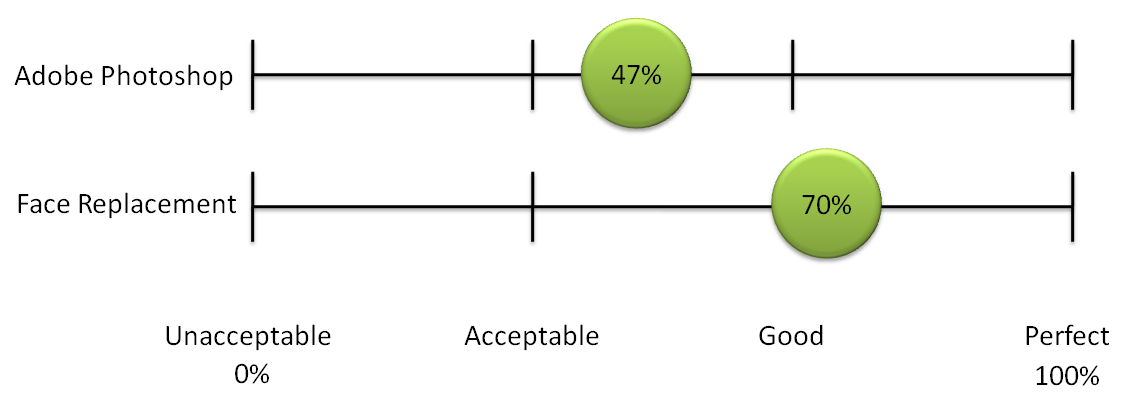
\includegraphics[width=12cm]{usersatisfaction.png}
   \caption{The Diagram Shows the Mean Average User Satisfaction Scores of both Adobe Photoshop and Face Replacement System}
   \label{fig:UserSatisfaction}
\end{figure}

From the results, we concluded that users can do face replacing by using the Face Replacement System approximately 2.5 times faster than the image retouching tool. We also concluded that users are more satisfied with the required time and the results from the Face Replacement System rather than doing it on their own by using the image retouching tool.

These are the examples of the output images which the volunteers created from both Adobe Photoshop and Face Replacement System. Note that the volunteers picked their own images to do this testing.

\begin{figure}[htb]
  \centering
  \subfloat[][Adobe Photoshop]{\label{fig:Photoshop2}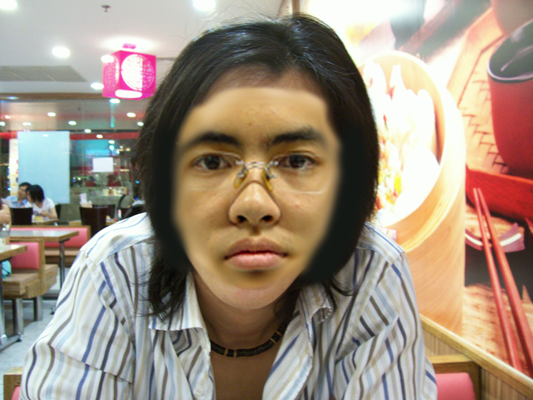
\includegraphics[width=0.3\textwidth]{PS.png}}
  \subfloat[][Face Replacement System]{\label{fig:FaceReplacement2}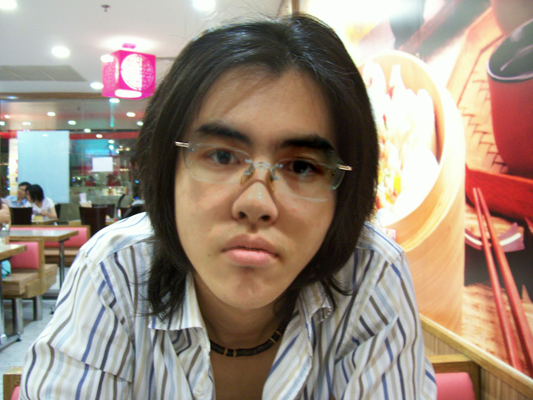
\includegraphics[width=0.3\textwidth]{FR.png}}
  \caption{The Output Images Created from Adobe Photoshop and the Face Replacement System}
  \label{fig:OutputImages}
\end{figure}

As shown in figure~\ref{fig:OutputImages}, the volunteer can locate the appropriate position of the facial features, but has difficulty in adjusting color and lighting when using Adobe Photoshop. However, our system can deal effectively with the color and lighting. We can see from other output images created from the Face Replacement System that the alignment is not as good as a human can do from Adobe Photoshop because of the lower accuracy of the face detector and the different appearances between the selected faces. Also, the volunteers are not familiar with system functionality, so they are not able to adjust the contour to be appropriate.

We also conducted the user interface evaluation by interviewing the volunteers about the system usage, including the user interface design. Figure~\ref{fig:InterfaceBefore} shows the user interface which is used for this evaluation.

\vspace{0.2in}\noindent We received the feedback from the volunteers as follows:

\begin{itemize}
\item The program does not provide the instruction for the users who use our system for the first time.
\item The color design of the interface is too translucent.
\item The option for selecting the techniques to do face replacement is described with technical terms which are difficult to understand for common users.
\item Users misunderstand the contour editing feature in that they thought they had to adjust those three pivots into eyes and mouth position, but the feature is intended for adjusting the contour in such a way that it does not to cross any face features.
\end{itemize}

\begin{figure}[htb]
   \centering
   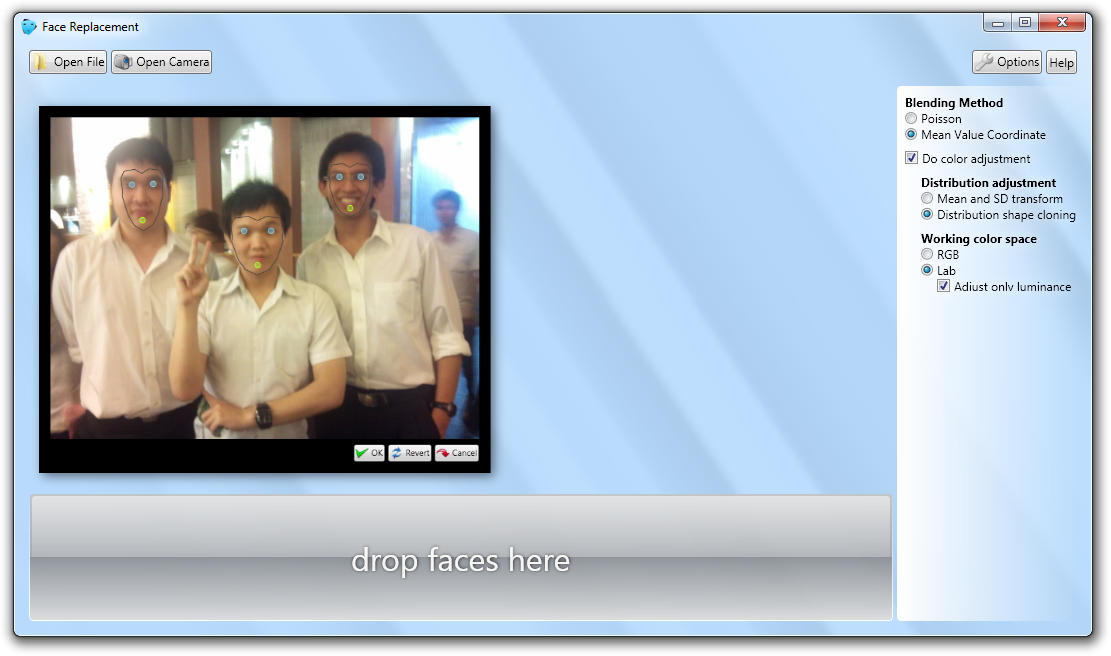
\includegraphics[width=14cm]{interface-before.png}
   \caption{The User Interface Version that Volunteers used for this Evaluation}
   \label{fig:InterfaceBefore}
\end{figure}

\noindent From the feedback, we improved the design and some functions of the system to be more effective as following:

\begin{figure}[htb]
   \centering
   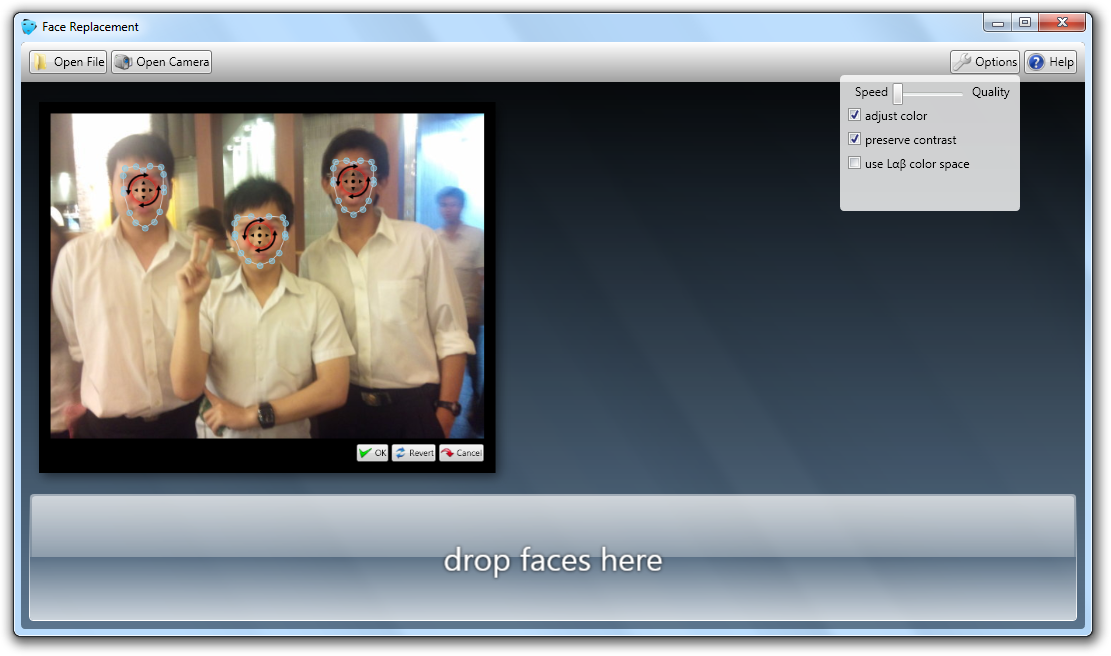
\includegraphics[width=14cm]{interface-after.png}
   \caption{The Recent Version of User Interface}
   \label{fig:InterfaceAfter}
\end{figure}

\begin{itemize}
\item We have created a Help feature providing the instruction of the program.
\item We have adjusted the color to be more opaque to look like the working space.
\item We have adjusted the option menu to be described with simple words and easy for common users to understand.
\item We have adjusted the contour editing feature to meet the user expectation. Users can translate the contour by grabbing the center circle pad, rotate by sliding around the center circle pad, and scale by moving each point of the contour points directly.
\end{itemize}

\section{Output Evaluation}
\hspace{0.5in}We conducted an evaluation to know how realistic the output images from the Face Replacement System will be compared to the output images from the image retouching tool. We invited another 5 volunteers to evaluate all the output images from the previous testing and score them using the percentages of the four scales of measurement as in the previous evaluation. The volunteers did not know which method was used to create each output image.

\begin{figure}[htb]
   \centering
   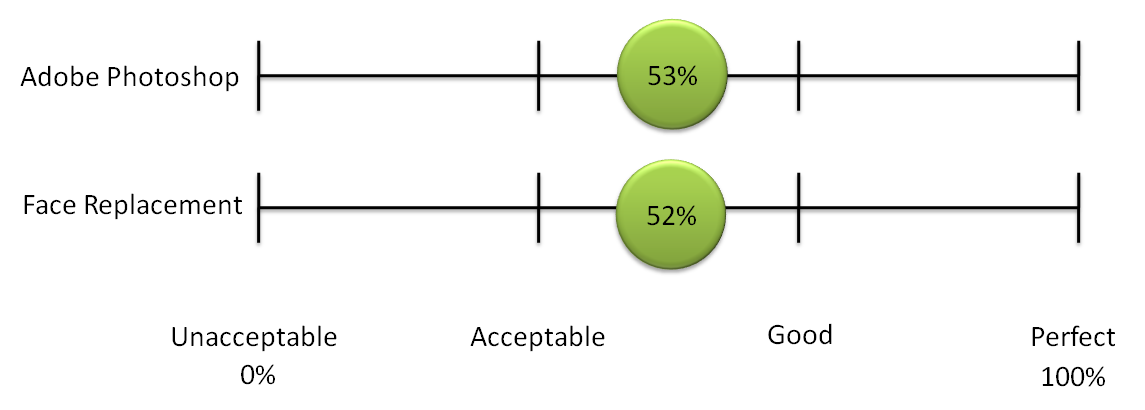
\includegraphics[width=12.5cm]{qualityscore.png}
   \caption{The Diagram Shows the Mean Average Quality Scores of both Adobe Photoshop and the Face Replacement System}
   \label{fig:QualityScore}
\end{figure}

From this evaluation, the quality score for the output images created using the image retouching tool was 53.54\%, whereas the score for the output images created using our system was 52\%. Both scores are in the Acceptable level.


We concluded that the face replacing output images from both methods are acceptable for participants. Both the quality scores of the output images using the image retouching tool and the Face Replacement System are approximately the same, which suggests our system can achieve the same output quality as human can do.

Note that the various image appearances the volunteers picked to do testing on and the various levels of image retouching skill can affect the required time and the quality of output images. The results may have been affected with these minor uncontrolled test variables.
